
\subsection{Validació 1: Primer Principi de la Termodinàmica} \label{sec:validacio_01}

Una primera manera de validar el codi és comprovar que els resultats que aquest produeix satisfan el Primer Principi de la Termodinàmica (PPT). De forma analítica, aquest ve donat per l'equació \eqref{eq:primer_principi_termodinamica_01}. No obstant això, és necessari particularitzar-lo per a cada tipus de node. Pels nodes interns el PPT és l'equació
\begin{equation}
	\rho_P V_P c_{p_P} \frac{T_P^{n+1} - T_P^n}{\Delta t} = 
	\beta \sum \dot{Q}_P^{n+1} + (1 - \beta) \sum \dot{Q}_P^n	
	\tag{\ref{eq:nodes_interns_eq_3}}
\end{equation}
on el flux de calor net està expressat en l'equació \eqref{eq:nodes_interns_fluxe_calor},
\begin{equation}
	\sum \dot{Q}_P^n =
	- \lambda_w \frac{T_P^n - T_W^n}{d_{PW}} S_w 
	+ \lambda_e \frac{T_E^n - T_P^n}{d_{PE}} S_e
	- \lambda_s \frac{T_P^n - T_S^n}{d_{PS}} S_s 
	+ \lambda_n \frac{T_N^n - T_P^n}{d_{PN}} S_n \tag{\ref{eq:nodes_interns_fluxe_calor}}
\end{equation}
Pels nodes superiors, el PPT és
\begin{equation} 
	\dot{q}_\text{flow} W \Delta x_P = 
	\lambda_s \frac{T_P^{n+1} - T_S^{n+1}}{d_{PS}} S_s
	\tag{\ref{eq:nodes_superiors_01}}
\end{equation}
i pels nodes esquerres ve donat per
\begin{equation}
	\alpha_g \left( T_P^{n+1} - T_g \right) S_\text{conv} = 
	\lambda_e \frac{T_E^{n+1} - T_P^{n+1}}{d_{PE}} S_e
	\tag{\ref{eq:nodes_esquerres_01}}
\end{equation}
En els nodes de la paret inferior hi ha la condició d'isoterma i en els de la paret dreta hi ha la condició de temperatura creixent. Com s'ha vist en les equacions de discretització, això implica que els coeficients de discretització pels nodes veïns són nuls i, en conseqüència, no hi ha flux de calor a través d'aquests nodes de contorn. Per tant en aquests nodes no és necessari comprovar el PPT.

Per portar a terme la verificació, s'escull una discretització uniforme en $x$, donada per la condició
\begin{equation}
	N_2 = \frac{6}{5} N_1, \quad N_1 \in 5 \z^+
\end{equation}
i uniforme en $y$, donada per
\begin{equation}
	L_2 = \frac{3}{4} L_1, \ 
	L_3 = \frac{1}{4} L_1, \quad
	L_1 \in 4 \z^+
\end{equation}
Es considera que amb $N_1 = 25$ i $L_1 = 28$ la malla és prou densa. Es pren un node representatiu de cada tipus i de cada . A la taula \ref{tab:nodes_verificacio} es listen els nodes de verificació. A la figura \ref{fig:nodes_verificacio} es mostra la posició dels nodes de verificació.

Quant a la discretització temporal, es prenen tres passos de temps $\Delta t$ diferents de $0.50 \ \second$, $1.00 \ \second$ i $10.00 \ \second$. Els esquemes d'integració temporal que s'utilitzen són l'esquema implícit $\left( \beta = 1 \right)$ i l'esquema de Crank--Nicolson $\left( \beta = 0.5 \right)$. No s'analitza l'esquema explícit $\left( \beta = 0 \right)$ ja que és condicionalment convergent i, en conseqüència, requereix de $\Delta t$ petit per funcionar correctament.

Per últim, pel que fa a la resolució numèrica del sistema d'equacions, s'estableix una tolerància per la convergència de $\delta = 10^{-12}$ i un nombre màxim d'iteracions $\textsf{itmax} = 500$. Si el mètode de Gauss--Seidel no convergeix en $\textsf{itmax}$ iteracions, aquest emet un missatge d'error.

En cada iteració i per a cada tipus de node, es recalculen els coeficients de discretització. A partir de les temperatures en $t^n$ i en $t^{n+1}$, es calculen els termes esquerre $\left( \mathrm{LHS} \right)$ i dret $\left( \mathrm{RHS} \right)$ de les equacions 
\eqref{eq:nodes_interns_eq_3}, \eqref{eq:nodes_superiors_01} i \eqref{eq:nodes_esquerres_01}. L'error és $\varepsilon_k = \abs{\mathrm{RHS}_k - \mathrm{LHS}_k}$.

\begin{table}[ht]
	\centering
	\begin{tabular}{llcc}
		\toprule[0.5mm]
		Node & Tipus & $(x,y) \ [\meter]$ & $[i,j]$ \\
		\midrule[0.25mm]
		1 & Intern $M_1$ 	& $(0.15, 0.15)$ & $[9,12]$ \\
		2 & Intern $M_2$ 	& $(0.65, 0.15)$ & $[34,12]$ \\
		3 & Intern $M_3$ 	& $(0.15, 0.75)$ & $[9,54]$ \\
		4 & Intern $M_4$ 	& $(0.65, 0.75)$ & $[34,54]$ \\
		5 & Superior $M_3$ 	& $(0.15, 0.80)$ & $[9,58]$ \\
		6 & Superior $M_4$ 	& $(0.65, 0.80)$ & $[34,58]$ \\
		7 & Esquerre $M_1$ 	& $(0.00, 0.15)$ & $[1,12]$ \\
		8 & Esquerre $M_3$ 	& $(0.00, 0.75)$ & $[1,54]$ \\
		\bottomrule[0.5mm]
	\end{tabular}
	\caption{Nodes per la verificació.}
	\label{tab:nodes_verificacio}
\end{table}

\begin{figure}[ht]
	\centering
	\begin{tikzpicture}
		% Fluido azul
		\fill[fill=cyan!70!white] (0,0) rectangle (5,4);
		\fill[fill=meatColor!70!white] (5,0) rectangle (11,7);
		\fill[fill=green!70!white] (0,4) rectangle (5,8);
		\fill[fill=red!70!white] (5,7) rectangle (11,8);
		\draw[black, line width=0.5mm] (5,0) -- ++(0,8);
		\draw[black, line width=0.5mm] (0,4) -- ++(5,0);
		\draw[black, line width=0.5mm] (5,7) -- ++(6,0);
		\draw[black, line width=0.5mm] (0,0) -- ++(11,0) -- ++(0,8) -- ++(-11,0) -- cycle;
		% Ejes
		\draw[->, black, line width=0.3mm] (-0.5,-1) -- (11.5,-1) node[above]{$x \ [\meter]$};
		\draw[->, black, line width=0.3mm] (-1,-0.5) -- (-1,8.5) node[right]{$y \ [\meter]$};
		% Marcas eje x
		\foreach \x in {0,...,11}
			\draw[black] (\x,-0.95) -- (\x,-1.05);
		\foreach \x in {0,...,11}
			\draw[black, dashed] (\x,-1) -- (\x,8);
		\node[black] at (0,-1.45) {$0.0$};
		\node[black] at (1,-1.45) {$0.1$};
		\node[black] at (2,-1.45) {$0.2$};
		\node[black] at (3,-1.45) {$0.3$};
		\node[black] at (4,-1.45) {$0.4$};
		\node[black] at (5,-1.45) {$0.5$};
		\node[black] at (6,-1.45) {$0.6$};
		\node[black] at (7,-1.45) {$0.7$};
		\node[black] at (8,-1.45) {$0.8$};
		\node[black] at (9,-1.45) {$0.9$};
		\node[black] at (10,-1.45) {$1.0$};
		\node[black] at (11,-1.45) {$1.1$};
		% Marcas eye y
		\foreach \y in {0,...,8}
			\draw[black, line width=0.3mm] (-0.95,\y) -- (-1.05,\y);
		\foreach \y in {0,...,8}
			\draw[black, dashed] (-1,\y) -- (11,\y);
		\node[black] at (-1.55,0) {$0.0$};
		\node[black] at (-1.55,1) {$0.1$};
		\node[black] at (-1.55,2) {$0.2$};
		\node[black] at (-1.55,3) {$0.3$};
		\node[black] at (-1.55,4) {$0.4$};
		\node[black] at (-1.55,5) {$0.5$};
		\node[black] at (-1.55,6) {$0.6$};
		\node[black] at (-1.55,7) {$0.7$};
		\node[black] at (-1.55,8) {$0.8$};
		% Nodo p1
		\filldraw[black] (1.5,1.5) circle(2pt) node[right]{$1$};
		\filldraw[black] (6.5,1.5) circle(2pt) node[right]{$2$};
		\filldraw[black] (1.5,7.5) circle(2pt) node[right]{$3$};
		\filldraw[black] (6.5,7.5) circle(2pt) node[right]{$4$};
		\filldraw[black] (1.5,8.0) circle(2pt) node[above]{$5$};
		\filldraw[black] (6.5,8.0) circle(2pt) node[above]{$6$};
		\filldraw[black] (0.0,1.5) circle(2pt) node[right]{$7$};
		\filldraw[black] (0.0,7.5) circle(2pt) node[right]{$8$};
	\end{tikzpicture}
	\caption{Posició dels nodes de verificació.}
	\label{fig:nodes_verificacio}
\end{figure}

\begin{figure}[ht]
	\centering
	\begin{subfigure}{.5\textwidth}
		\centering
		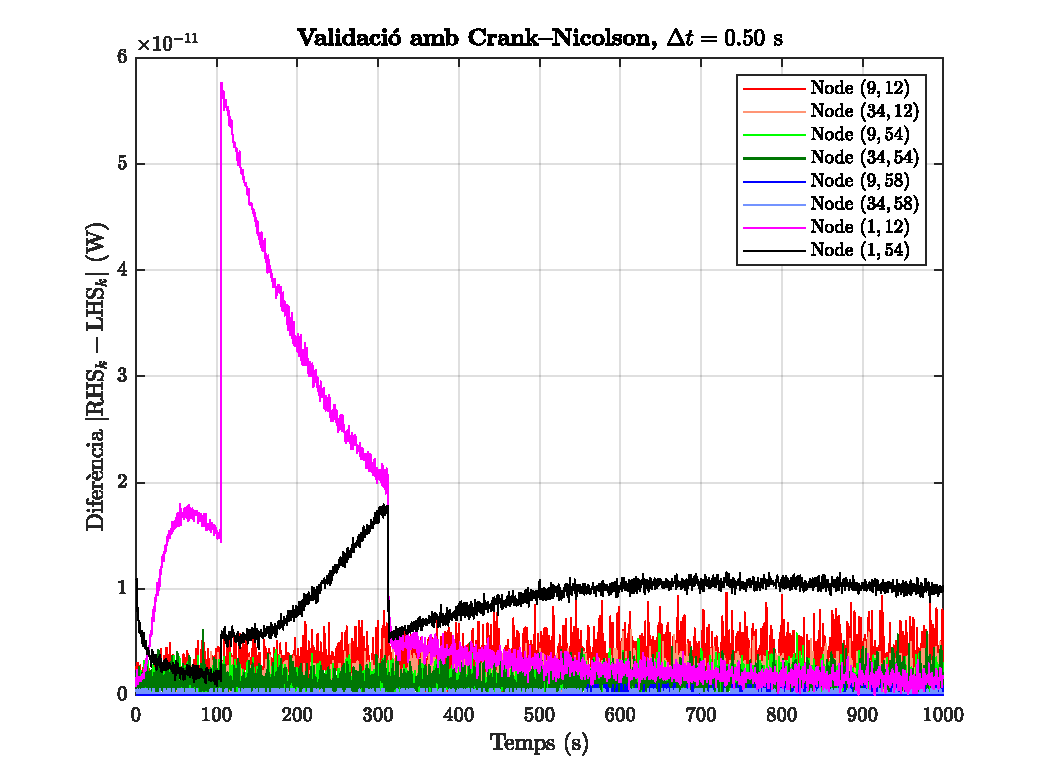
\includegraphics[width=.95\linewidth]{imagenes/03_validacio/validacio_01.pdf}
		\vspace{-7pt}
		\caption{$\Delta t = 0.50 \ \second$, $t_\text{max} = 1000 \ \second$.}
		\label{fig:validacio_01}
%		\vspace{10pt}
	\end{subfigure}%
	\begin{subfigure}{.5\textwidth}
		\centering
		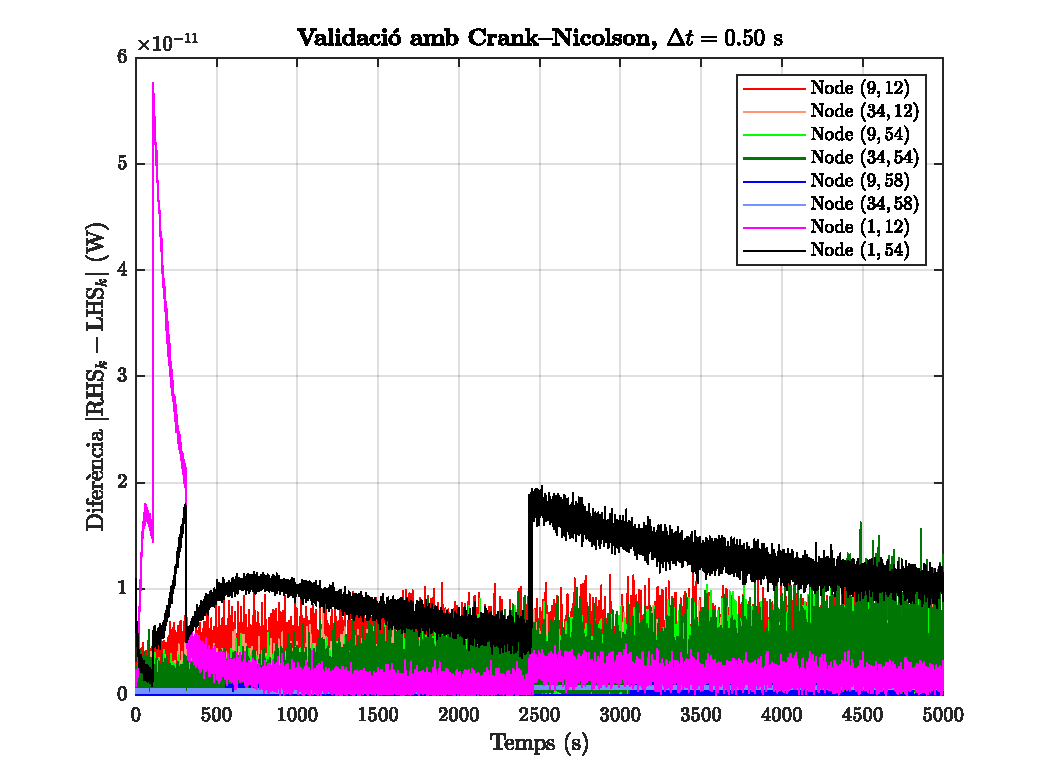
\includegraphics[width=.95\linewidth]{imagenes/03_validacio/validacio_02.pdf}
		\vspace{-7pt}
		\caption{$\Delta t = 0.50 \ \second$, $t_\text{max} = 5000 \ \second$.}
		\label{fig:validacio_02}
%		\vspace{10pt}
	\end{subfigure}
	\begin{subfigure}{.5\textwidth}
		\centering
		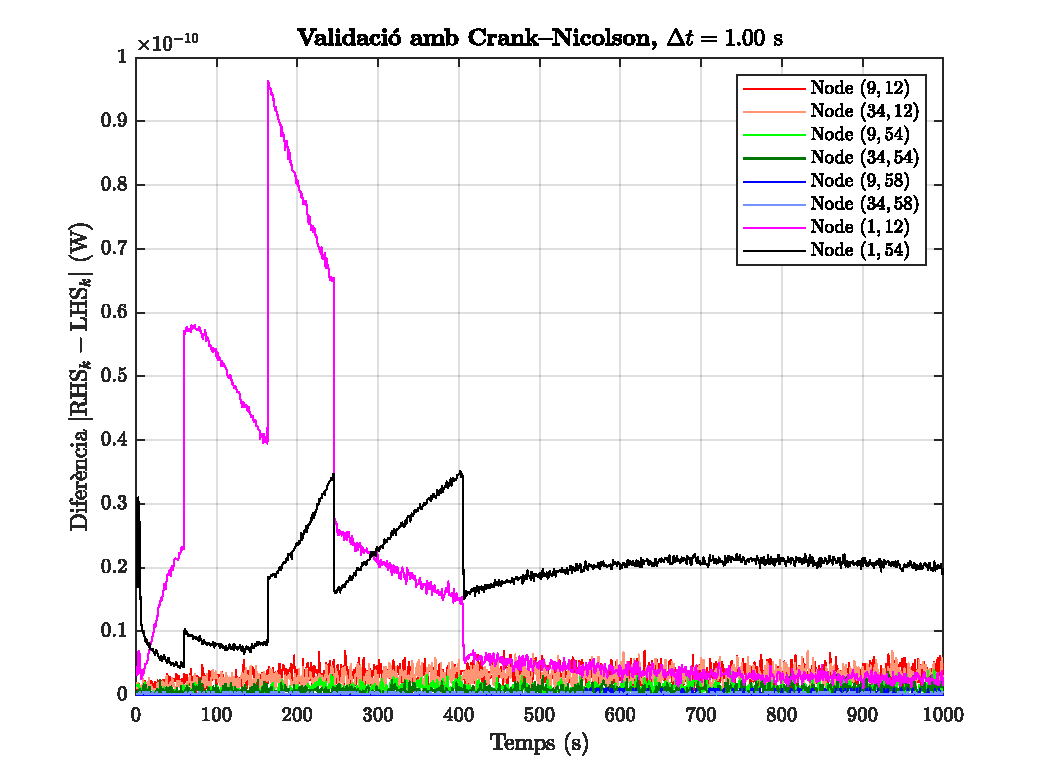
\includegraphics[width=.95\linewidth]{imagenes/03_validacio/validacio_03.pdf}
		\vspace{-7pt}
		\caption{$\Delta t = 1.00 \ \second$, $t_\text{max} = 1000 \ \second$.}
		\label{fig:validacio_03}
%		\vspace{10pt}
	\end{subfigure}%
	\begin{subfigure}{.5\textwidth}
		\centering
		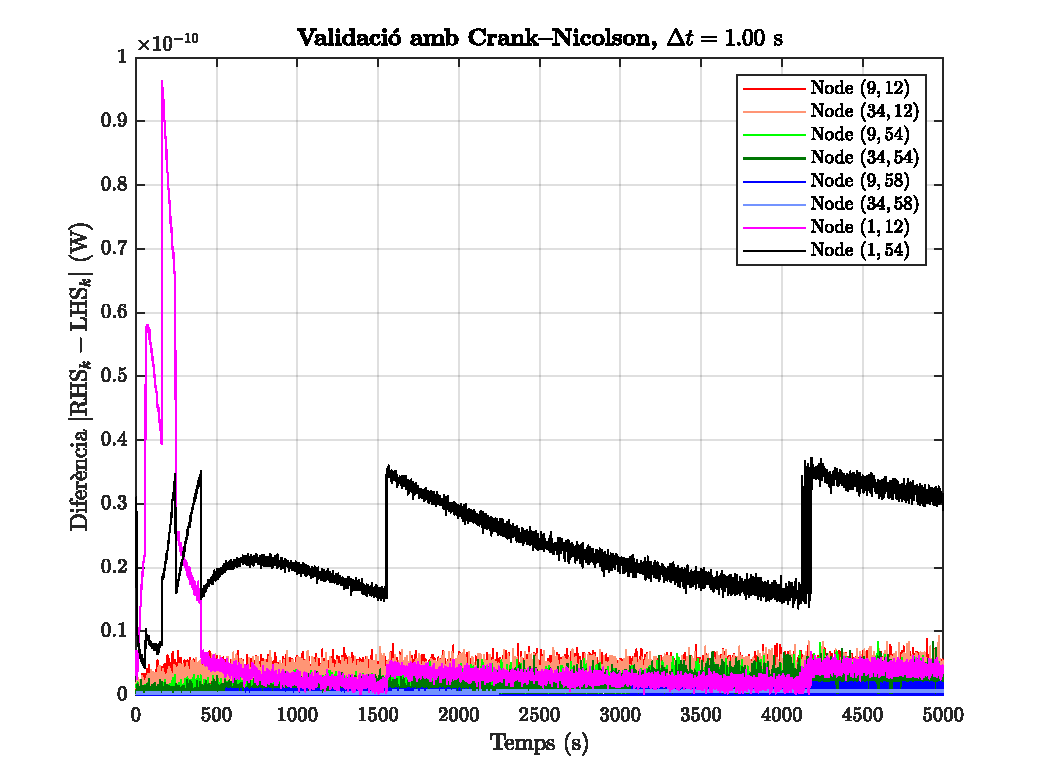
\includegraphics[width=.95\linewidth]{imagenes/03_validacio/validacio_04.pdf}
		\vspace{-7pt}
		\caption{$\Delta t = 1.00 \ \second$, $t_\text{max} = 5000 \ \second$.}
		\label{fig:validacio_04}
%		\vspace{10pt}
	\end{subfigure}
	\begin{subfigure}{.5\textwidth}
		\centering
		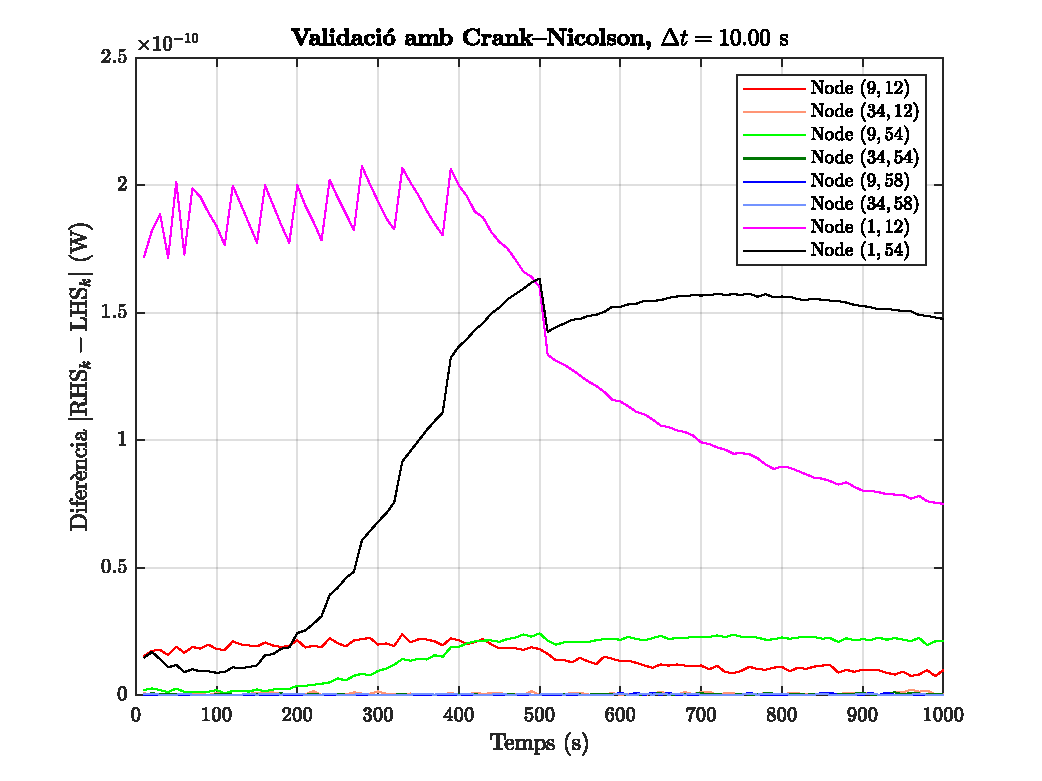
\includegraphics[width=.95\linewidth]{imagenes/03_validacio/validacio_05.pdf}
		\vspace{-7pt}
		\caption{$\Delta t = 10.00 \ \second$, $t_\text{max} = 1000 \ \second$.}
		\label{fig:validacio_05}
%		\vspace{10pt}
	\end{subfigure}%
	\begin{subfigure}{.5\textwidth}
		\centering
		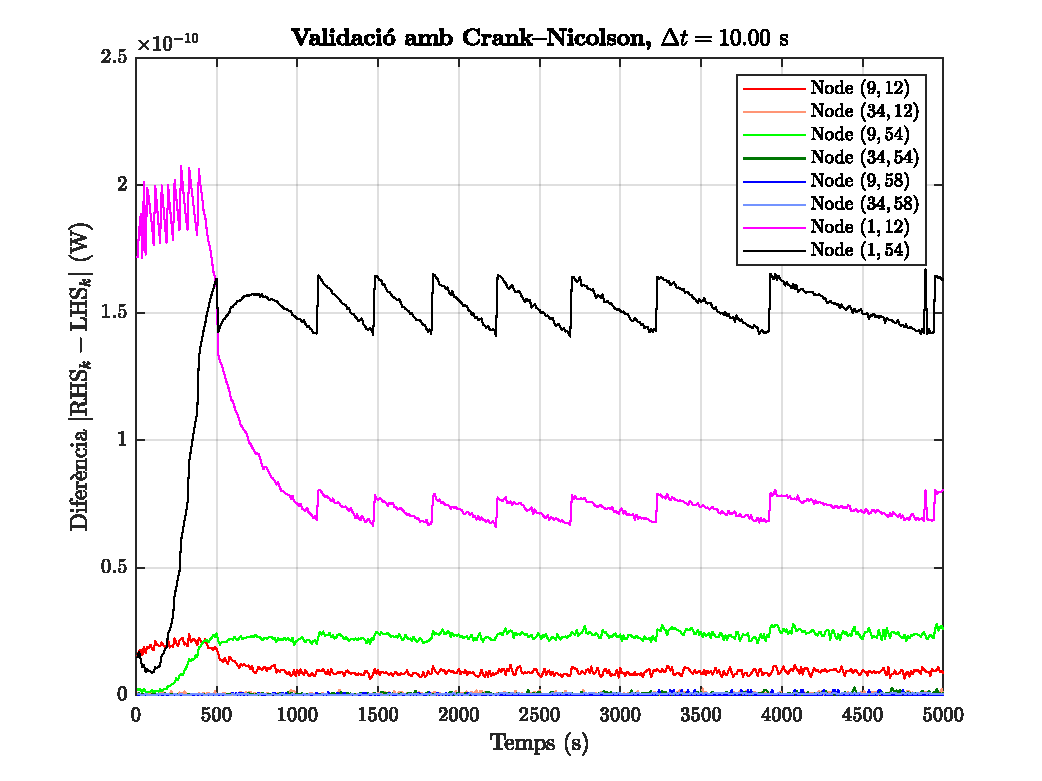
\includegraphics[width=.95\linewidth]{imagenes/03_validacio/validacio_06.pdf}
		\vspace{-7pt}
		\caption{$\Delta t = 10.00 \ \second$, $t_\text{max} = 5000 \ \second$.}
		\label{fig:validacio_06}
	\end{subfigure}
	\caption{Validació amb esquema de Crank--Nicolson. Cada fila es correspon amb un $\Delta t$ diferent. La simulació en tots casos ha estat fins $t_\text{max} = 5000 \ \second$. A la columna esquerra es mostra el detall dels primers $1000 \ \second$ de simulació. Com s'observa, a mida que creix $\Delta t$, també creix l'error. No obstant això, en tots els casos es compleix que $\varepsilon_k < 0.5 \ \times 10^{-9}$. Com resulta intuïtiu, la millor aproximació s'obté amb $\Delta t = 0.50 \ \second$. En tots els casos els nodes amb major error són els nodes $[1,12]$ i $[1,54]$ de la paret esquerre. Així mateix, s'aprecia certa periodicitat en la variació de l'error del node $[1,54]$.}
	\label{fig:validacio_crank_nicolson}
\end{figure}


\begin{figure}[ht]
	\centering
	\begin{subfigure}{.5\textwidth}
		\centering
		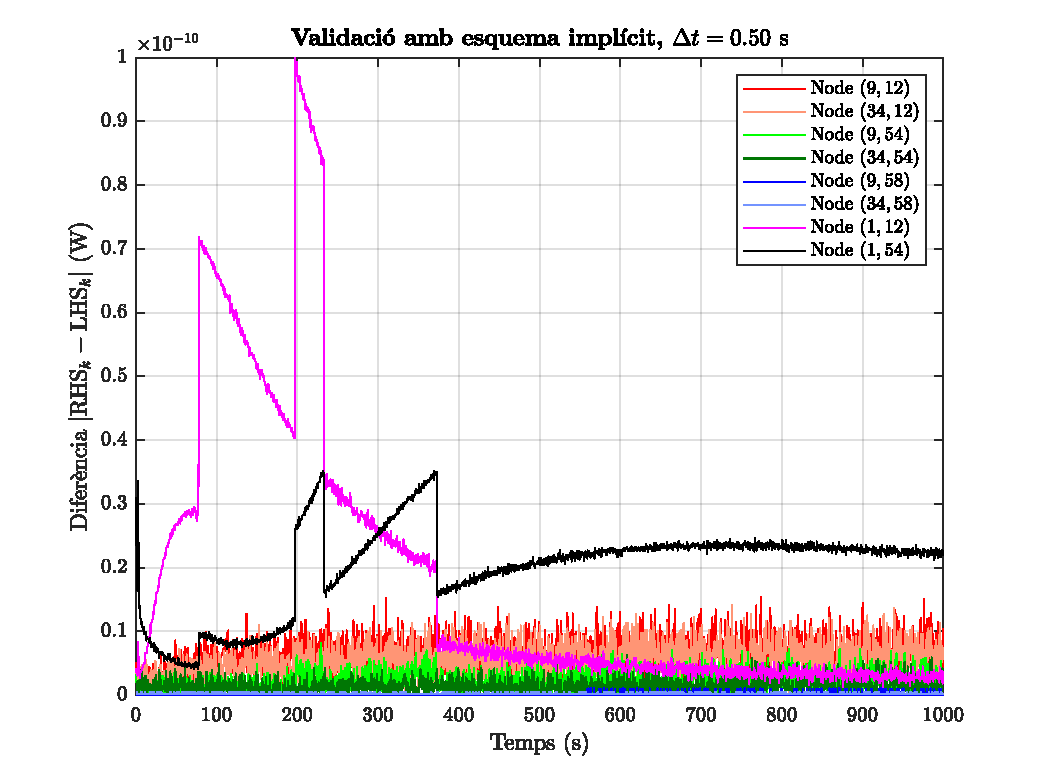
\includegraphics[width=.95\linewidth]{imagenes/03_validacio/validacio_07.pdf}
		\vspace{-7pt}
		\caption{$\Delta t = 0.50 \ \second$, $t_\text{max} = 1000 \ \second$.}
		\label{fig:validacio_07}
%		\vspace{10pt}
	\end{subfigure}%
	\begin{subfigure}{.5\textwidth}
		\centering
		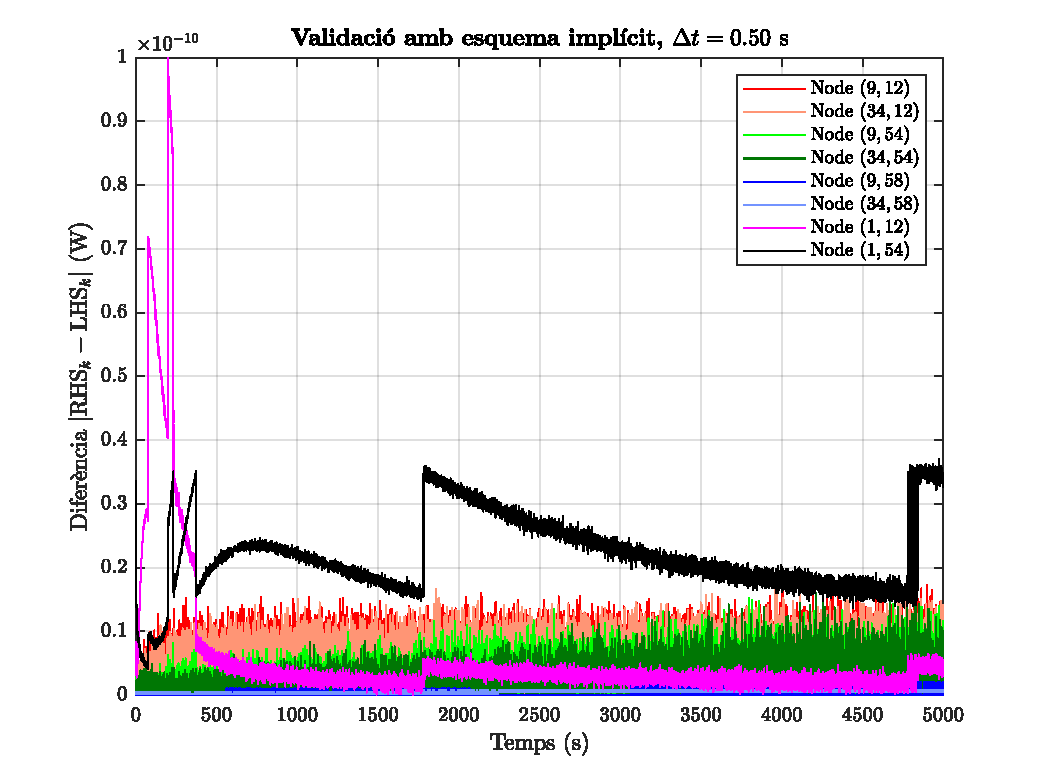
\includegraphics[width=.95\linewidth]{imagenes/03_validacio/validacio_08.pdf}
		\vspace{-7pt}
		\caption{$\Delta t = 0.50 \ \second$, $t_\text{max} = 5000 \ \second$.}
		\label{fig:validacio_08}
%		\vspace{10pt}
	\end{subfigure}
	\begin{subfigure}{.5\textwidth}
		\centering
		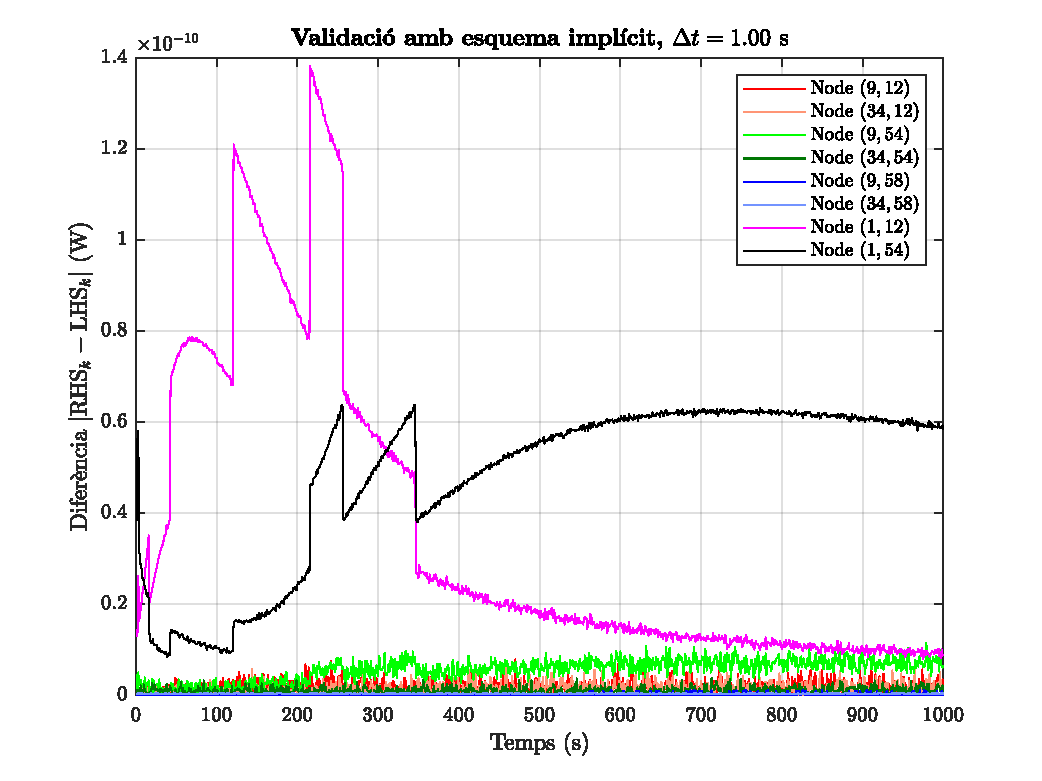
\includegraphics[width=.95\linewidth]{imagenes/03_validacio/validacio_09.pdf}
		\vspace{-7pt}
		\caption{$\Delta t = 1.00 \ \second$, $t_\text{max} = 1000 \ \second$.}
		\label{fig:validacio_09}
%		\vspace{10pt}
	\end{subfigure}%
	\begin{subfigure}{.5\textwidth}
		\centering
		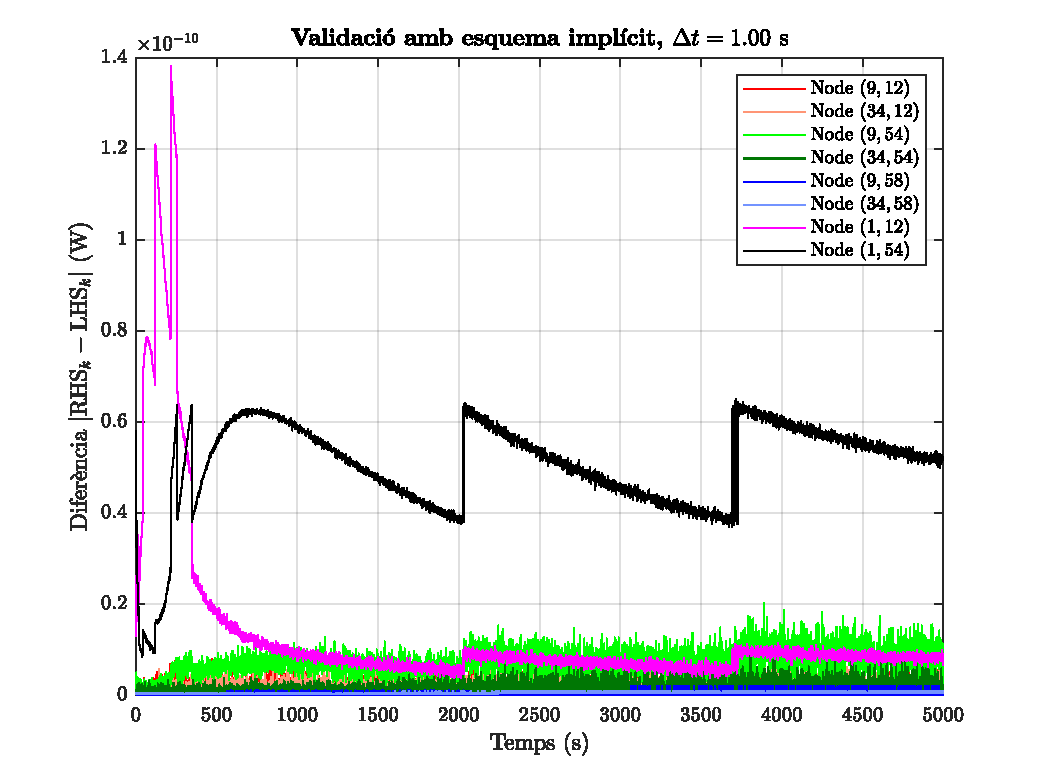
\includegraphics[width=.95\linewidth]{imagenes/03_validacio/validacio_10.pdf}
		\vspace{-7pt}
		\caption{$\Delta t = 1.00 \ \second$, $t_\text{max} = 5000 \ \second$.}
		\label{fig:validacio_10}
%		\vspace{10pt}
	\end{subfigure}
	\begin{subfigure}{.5\textwidth}
		\centering
		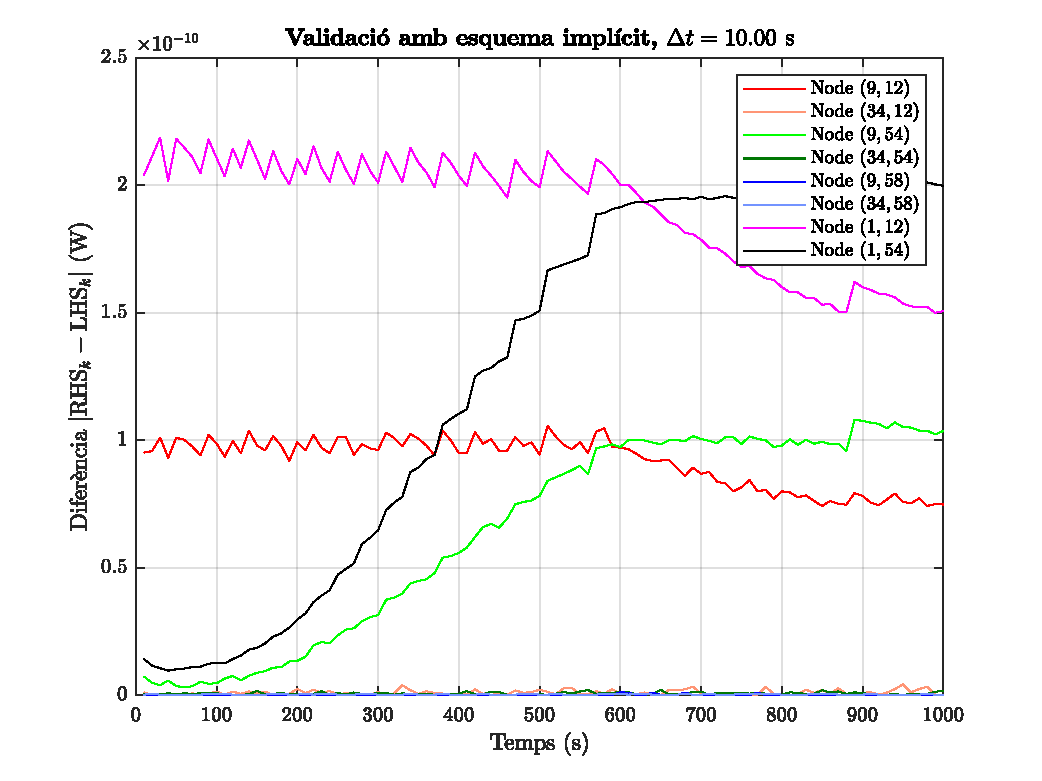
\includegraphics[width=.95\linewidth]{imagenes/03_validacio/validacio_11.pdf}
		\vspace{-7pt}
		\caption{$\Delta t = 10.00 \ \second$, $t_\text{max} = 1000 \ \second$.}
		\label{fig:validacio_11}
%		\vspace{10pt}
	\end{subfigure}%
	\begin{subfigure}{.5\textwidth}
		\centering
		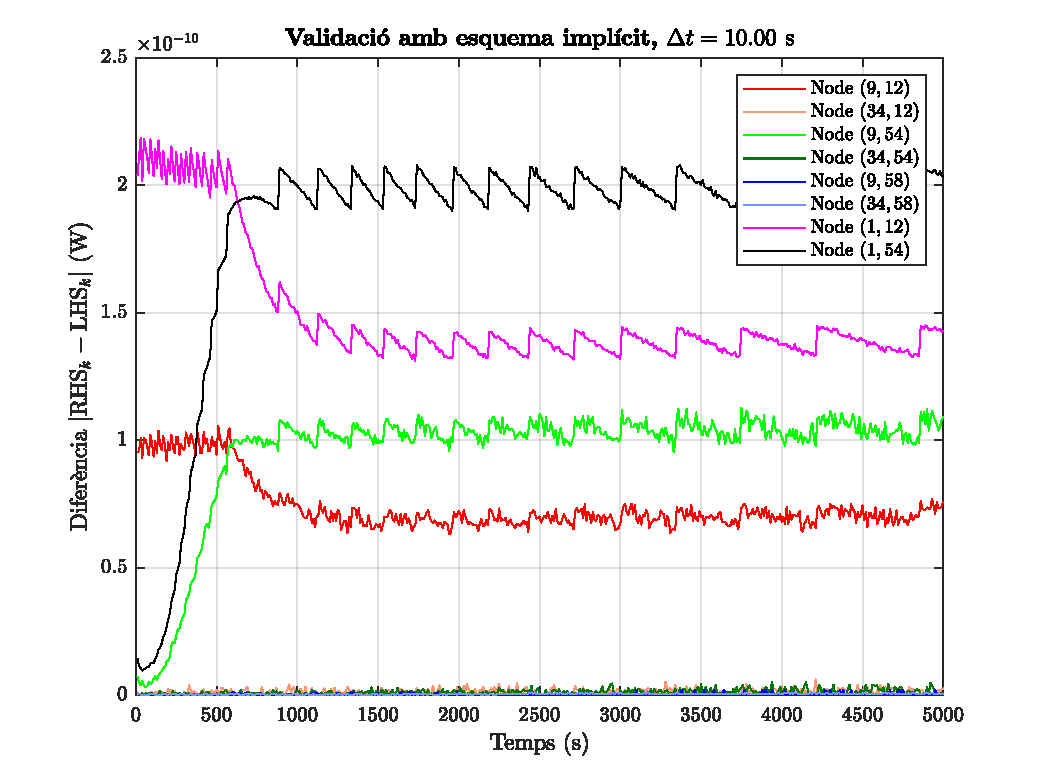
\includegraphics[width=.95\linewidth]{imagenes/03_validacio/validacio_12.pdf}
		\vspace{-7pt}
		\caption{$\Delta t = 10.00 \ \second$, $t_\text{max} = 5000 \ \second$.}
		\label{fig:validacio_12}
	\end{subfigure}
	\caption{Validació amb esquema implícit. La distribució de gràfiques és igual a l'anterior. S'aprecia que en aquest cas l'error augmenta en comparació amb l'esquema de Crank--Nicolson. Això pot ser degut al diferent ordre que donen ambdues aproximacions.}
	\label{fig:validacio_implicit}
\end{figure}



